\section{VCVS Voltage Gain}

\subsection{Exact Closed-Loop Voltage Gain}
\begin{frame}{Exact Closed-Loop Voltage Gain}
	\begin{multicols}{2}
		\begin{figure}
			\centering
			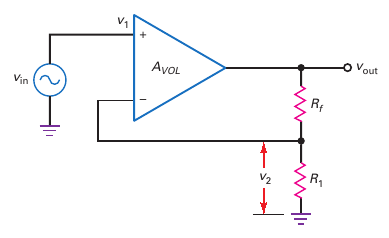
\includegraphics[width=0.9\linewidth]{gambar/fig-17.03}
			\caption{VCVS Amplifier}
			\label{fig-17.03}
		\end{figure}
	\columnbreak
	\begin{itemize}
		\item Feedback fraction atau feedback attenuation factor:
		\begin{equation}\label{pers-17.01}
			B = \frac{v_2}{v_{out}}
		\end{equation}
		\item Closed-loop voltage gain:
		\begin{equation}\label{pers-17.02}
			A_{v(CL)} = \frac{A_{VOL}}{1 + A_{VOL}B}
		\end{equation}
		\item Exact closed-loop voltage gain:
		\begin{equation}\label{pers-17.03}
			A_v = A_{v(CL)} = \frac{A_{VOL}}{1 + A_{VOL}B}
		\end{equation}
	\end{itemize}
	\end{multicols}
\end{frame}

\subsection{Loop Gain}
\begin{frame}{Loop Gain}
	\begin{itemize}
		\item Loop gain: $ A_{VOL} B$
		\item Disebut loop gain karena voltage gain dari forward dan feedback path
		\item Loop gain sangat penting dalam mendesain negative-feedback amplifier
		\item Loop gain dibuat sangat besar
		\item Semakin besar loop gain maka semakin baik karena menstabilkan voltage gain dan memperbaiki gain stability, distortion, offset, impedansi input dan impedansi output
	\end{itemize}
\end{frame}

\subsection{Ideal Closed-Loop VOltage Gain}
\begin{frame}{Ideal Closed-Loop VOltage Gain}
	\begin{itemize}
		\item VCVS bekerja dengan baik jika loop gain jauh lebih besar daripada unity
	\end{itemize}

	\begin{equation}\label{pers-17.04}
		A_v = \frac{A_{VOL}}{1 + A_{VOL} B} \cong \frac{A_{VOL}}{A_{VOL} B} = \frac{1}{B}
	\end{equation}

	\begin{itemize}
		\item Percent error antara nilai ideal dan exact:
	\end{itemize}

	\begin{equation}\label{pers-17.05}
		\% Error = \frac{100\%}{1 + A_{VOL} B}
	\end{equation}
\end{frame}

\subsection{Menggunakan Persamaan Ideal}
\begin{frame}{Menggunakan Persamaan Ideal}
	\begin{itemize}
		\item Feedback fraction:
		\begin{equation}\label{pers-17.06}
			V = \frac{v_2}{v_{out}} = \frac{R_1}{R_1 + R_f}
		\end{equation}
		\[ A_v \cong \frac{1}{B} = \frac{R_1 + R_f}{R_1} = \frac{R_f}{R_1} + 1 \]
	\end{itemize}
\end{frame}

\subsection{Contoh Soal 3.4}
\begin{frame}{Contoh Soal 3.4}
	content...
\end{frame}